% -----------------------------------------------------------------------------
%                                     HEADER                                    
% -----------------------------------------------------------------------------
\documentclass[a4paper, 10pt]{article}
\usepackage{jheppub}
\usepackage[T1]{fontenc}
\usepackage{colortbl,xcolor,float}
\definecolor{orange}{rgb}{1,0.5,0}
% -----------------------------------------------------------------------------
%                                   COVER PAGE                                  
% -----------------------------------------------------------------------------
\title{{
\includegraphics[scale=.4]{logo.png}}\ The LaTeX report}

\author{Generated by jhkim on 13 February 2020, 17:39:51}

\abstract{
  This report has been generated automatically
  by {\sc MadAnalysis} 5.\\$~$\\ 
  Please cite:\\ 
  \begin{quote}
    \textbf{E.~Conte, B.~Fuks and G.~Serret},\\ 
    \textit{MadAnalysis 5, A User-Friendly
    Framework for Collider Phenomenology},\\ 
    Comput. Phys. Commun. {\bf 184} (2013) 222-256,\\
    arXiv:1206.1599 [hep-ph].\\ 
  \end{quote}
  To contact us:\\ 
  \begin{quote}
    \textbf{http://madanalysis.irmp.ucl.ac.be}\\
    \textbf{ma5team@iphc.cnrs.fr}\\
  \end{quote}
}

% -----------------------------------------------------------------------------
%                                 BEGIN DOCUMENT                                
% -----------------------------------------------------------------------------
\begin{document}
\maketitle
\flushbottom

% -----------------------------------------------------------------------------
%                                 SECTION Setup                                 
% -----------------------------------------------------------------------------
\newpage
\section{ Setup}

\subsection{ Command history}

\texttt{ma5>install samples\\
}
\texttt{ }\texttt{ }\texttt{ma5>display\_multiparticles\\
}
\texttt{ }\texttt{ }\texttt{ma5>define mu = mu+ mu-\\
}
\texttt{ }\texttt{ }\texttt{ma5>import samples/\-ttbar\_*.lhe.gz\\
}
\texttt{ }\texttt{ }\texttt{ma5>plot PT(mu)\\
}
\texttt{ }\texttt{ }\texttt{ma5>reject plot PT(mu) < 40\\
}
\texttt{ }\texttt{ }\texttt{ma5>reject PT(mu) < 40\\
}
\texttt{ }\texttt{ }\texttt{ma5>plot PT(mu)\\
}
\texttt{ }\texttt{ }\texttt{ma5>submit\\
}
\texttt{ }\texttt{ }\subsection{ Configuration}

\begin{itemize}
  \item MadAnalysis version 1.8.40 (2020/\-01/\-29).
   \item Histograms given for an integrated luminosity of \textcolor{blue}{10}\textcolor{blue}{ fb}$^{\textcolor{blue}{-1}}$\textcolor{blue}{.}
\textcolor{blue}{}
\end{itemize}
% -----------------------------------------------------------------------------
%                                SECTION Datasets                               
% -----------------------------------------------------------------------------
\newpage
\section{ Datasets}

\subsection{ defaultset}

\begin{itemize}
  \item Sample consisting of: \textcolor{blue}{signal}  events.
   \item Generated events: \textcolor{blue}{3000 }  events.
   \item Normalization to the luminosity: \textcolor{blue}{146623}\textcolor{blue}{ +/\-- }\textcolor{blue}{1054 }  events.
   \item\textcolor{red}{Ratio (event weight): }\textcolor{red}{48 }\textcolor{red}{ - warning: please generate more events (weight larger than 1)!}
\textcolor{red}{}
\end{itemize}
\begin{table}[H]
  \begin{center}
    \begin{tabular}{|m{55.0mm}|m{25.0mm}|m{30.0mm}|m{30.0mm}|}
      \hline
      {\cellcolor{yellow}         Paths to the event files}& {\cellcolor{yellow}         Nr. of events}& {\cellcolor{yellow}         Cross section (pb)}& {\cellcolor{yellow}         Negative wgts (\%)}\\
      \hline
      {\cellcolor{white}          samples/\-ttbar\_sl\_1.lhe.gz}& {\cellcolor{white}          1000}& {\cellcolor{white}          15.4 @ 0.74\%}& {\cellcolor{white}          0.0}\\
      \hline
      {\cellcolor{white}          samples/\-ttbar\_sl\_2.lhe.gz}& {\cellcolor{white}          1000}& {\cellcolor{white}          15.2 @ 0.66\%}& {\cellcolor{white}          0.0}\\
      \hline
      {\cellcolor{white}          samples/\-ttbar\_fh.lhe.gz}& {\cellcolor{white}          1000}& {\cellcolor{white}          13.3 @ 2.1\%}& {\cellcolor{white}          0.0}\\
      \hline
      {\cellcolor{white}         \textcolor{blue}{Sum}}& {\cellcolor{white}         \textcolor{blue}{3000}}& {\cellcolor{white}         \textcolor{blue}{14.7 @ 0.72\%}}& {\cellcolor{white}         \textcolor{blue}{0.0}}\\
\hline
    \end{tabular}
  \end{center}
\end{table}

% -----------------------------------------------------------------------------
%                            SECTION Histos and cuts                            
% -----------------------------------------------------------------------------
\newpage
\section{ Histos and cuts}

\subsection{ Histogram 1}

\textbf{* Plot: PT ( mu ) }\\
   \begin{table}[H]
  \begin{center}
    \begin{tabular}{|m{23.0mm}|m{23.0mm}|m{18.0mm}|m{19.0mm}|m{19.0mm}|m{19.0mm}|m{19.0mm}|}
      \hline
      {\cellcolor{yellow}         Dataset}& {\cellcolor{yellow}         Integral}& {\cellcolor{yellow}         Entries per event}& {\cellcolor{yellow}         Mean}& {\cellcolor{yellow}         RMS}& {\cellcolor{yellow}         \% underflow}& {\cellcolor{yellow}         \% overflow}\\
      \hline
      {\cellcolor{white}         defaultset}& {\cellcolor{white}         48239}& {\cellcolor{white}         1.0}& {\cellcolor{white}         49.6728}& {\cellcolor{white}         34.55}& {\cellcolor{green}         0.0}& {\cellcolor{green}         0.0}\\
\hline
    \end{tabular}
  \end{center}
\end{table}

\begin{figure}[H]
  \begin{center}
    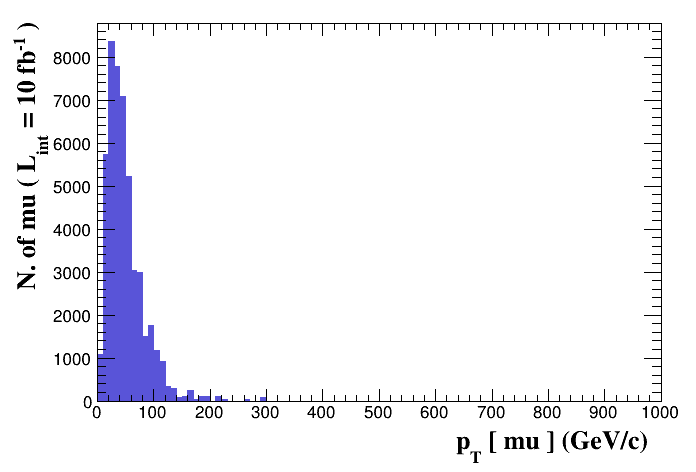
\includegraphics[scale=0.45]{selection_0.png}\\
\caption{   }
  \end{center}
\end{figure}
      \newpage
\subsection{Cut 1}

\textbf{* Cut: reject PT ( mu ) < 40.0}\\
   \begin{table}[H]
  \begin{center}
    \begin{tabular}{|m{20.0mm}|m{27.0mm}|m{27.0mm}|m{33.0mm}|m{32.0mm}|}
      \hline
      {\cellcolor{yellow}         Dataset}& {\cellcolor{yellow}         Events kept:
          K}& {\cellcolor{yellow}         Rejected events:
          R}& {\cellcolor{yellow}         Efficiency:
          K /\- (K + R)}& {\cellcolor{yellow}         Cumul. efficiency:
          K /\- Initial}\\
      \hline
      {\cellcolor{white}         defaultset}& {\cellcolor{white}         122632 +/\-- 892}& {\cellcolor{white}         23991 +/\-- 223}& {\cellcolor{white}         0.836374 +/\-- 0.000966}& {\cellcolor{white}         0.836374 +/\-- 0.000966}\\
\hline
    \end{tabular}
  \end{center}
\end{table}

   \newpage
\subsection{ Histogram 2}

\textbf{* Plot: PT ( mu ) }\\
   \begin{table}[H]
  \begin{center}
    \begin{tabular}{|m{23.0mm}|m{23.0mm}|m{18.0mm}|m{19.0mm}|m{19.0mm}|m{19.0mm}|m{19.0mm}|}
      \hline
      {\cellcolor{yellow}         Dataset}& {\cellcolor{yellow}         Integral}& {\cellcolor{yellow}         Entries per event}& {\cellcolor{yellow}         Mean}& {\cellcolor{yellow}         RMS}& {\cellcolor{yellow}         \% underflow}& {\cellcolor{yellow}         \% overflow}\\
      \hline
      {\cellcolor{white}         defaultset}& {\cellcolor{white}         25316}& {\cellcolor{white}         1.0}& {\cellcolor{white}         71.8934}& {\cellcolor{white}         34.18}& {\cellcolor{green}         0.0}& {\cellcolor{green}         0.0}\\
\hline
    \end{tabular}
  \end{center}
\end{table}

\begin{figure}[H]
  \begin{center}
    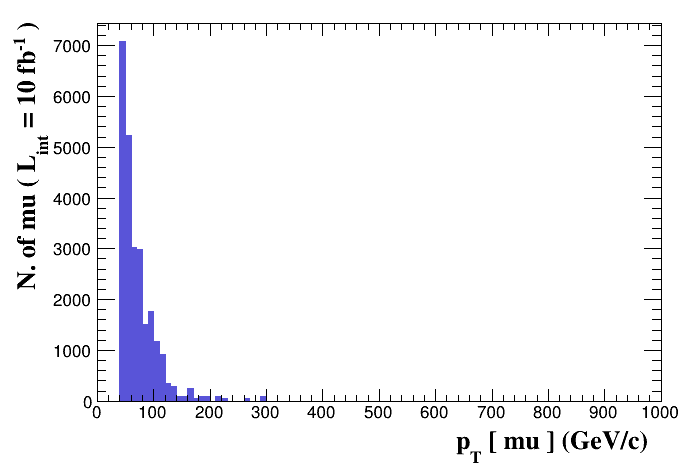
\includegraphics[scale=0.45]{selection_1.png}\\
\caption{   }
  \end{center}
\end{figure}
      % -----------------------------------------------------------------------------
%                                SECTION Summary                                
% -----------------------------------------------------------------------------
\newpage
\section{ Summary}

\subsection{Cut-flow charts}

\begin{itemize}
  \item How to compare signal (S) and background (B): \textcolor{blue}{S/\-sqrt(S+B)} .
   \item Object definition selections are indicated in cyan.  \item Reject and select are indicated by 'REJ' and 'SEL' respectively
\end{itemize}
\begin{table}[H]
  \begin{center}
    \begin{tabular}{|m{36.0mm}|m{36.0mm}|m{36.0mm}|m{33.0mm}|}
      \hline
      {\cellcolor{yellow}        Cuts}& {\cellcolor{yellow}         Signal (S)}& {\cellcolor{yellow}         Background (B)}& {\cellcolor{yellow}         S vs B}\\
      \hline
      {\cellcolor{white}         Initial (no cut)}& {\cellcolor{white}         146623 +/\-- 1053}& {\cellcolor{white}         }& {\cellcolor{white}         }\\
      \hline
      {\cellcolor{white} REJ: PT ( mu ) < 40.0}& {\cellcolor{white}         122632 +/\-- 892}& {\cellcolor{white}         }& {\cellcolor{white}         }\\
\hline
    \end{tabular}
  \end{center}
\end{table}

\end{document}
